\section{Introduction}
\subsection{Current use case}
Visual inspection is inherent part of railway track monitoring activities to ensure proper
condition of the infrastructure and thus provide a safe railway operation.
Besides many possibilities of track monitoring, such as ultrasonic or laser-based measurements,
vehicle riding parameters (or ride comfort) analysis, still visual inspection is evitable.
During regular track investigations video recordings done from the rails itself from different
views which allows off-line evaluation.
An accurate and reliable evaluation method is desirable that would help the maintenance personnel
to automatically find the track failures in these video recordings, or at least limit the duration
of these to reduce required human resources.
Usually 60-70 rail defects found every year during hundreds of kilometers of inspection rides.
This already highlights the difficulties of the given problem.

\subsection{Railway track fault detection}
Image based railway track fault detection is narrowed down to certain set of faults in terms of applied methods.
There are two key areas, the first one is surface defect detection and the second one is the
identification of missing elements of the rail, mostly focusing on fastening elements.

Several tools are already applied with good success, starting from pure image processing approaches
(edge detection, threshold application, etc.) up to traditional and machine learning based algorithms
(e.g.: SVM, random forests).
Image processing offers the opportunity to apply convolutional neural networks that could describe
the content of these images in a compressed format capturing their main features both in (image-wise)
local and global scale.
These compressions can be used for further tasks such as classification or anomaly detection.

A deeper overview of the literature is provided in \cite{tomcom_mathemathical_2022} with examples
of the key areas and applied tools.

\subsection{Previous work and results}
Current research started as part of the studies on the Mathematics Expert in
Data Analytics and Machine Learning postgraduate specialization program \cite{_ai&ml_}
held by the AI Research Group of Eötvös Lóránd University \cite{_ai_}.
During the one-year program a thesis work has to be created that is often
preceded by a modeling practice in the first semester.
This project follows the same approach as railway track fault detection models
were already built in the first semester.
However, the characteristics of the dataset used at that time did not allow a
successful application of a model however valuable experience is gained together
with a boost of motivation to follow up the topic and deepen the knowledge in the
mentioned field.

During the first semester basic convolutional neural networks were built with classification
head to identify images with defective railway tracks \cite{tomcom_mathemathical_2022}.
LeNet-5, AlexNet, VGG16 and ResNet50 were applied, partially utilizing transfer learning as well
(indicated with \lstinline{_p} suffix in the following).

The dataset was taken from the Kaggle webpage \cite{_railway_} consisting of a limited
number of images with defective and non-defective railway tracks that were already annotated.
The images combine a high variety of failures (such as rail cracks, missing fastening elements,
complete track failures) with very limited examples.
Additionally, the photos are taken from a wide range and angle, lacking any kind of standard positioning.
This leads to a very specific dataset.
Furthermore, the low amount of images and imbalanced characteristics of the dataset limits
the possibility of effectively apply neural networks due to the high number of parameters
that need to be optimized in such models.

The results of the modeling is shown on Figure \ref{fig:Kaggle_results}, where the performance of
different bootstrapped models on the splits of the dataset is given.
Bootstrapping technique was applied in the end to investigate how far the validation and test set could
describe the initial training dataset.
As shown in the figure, the high range of the obtained results of each model already indicates
that the distribution of the training images differ from the other splits of the dataset.

\begin{figure}[!ht]
    \centering
    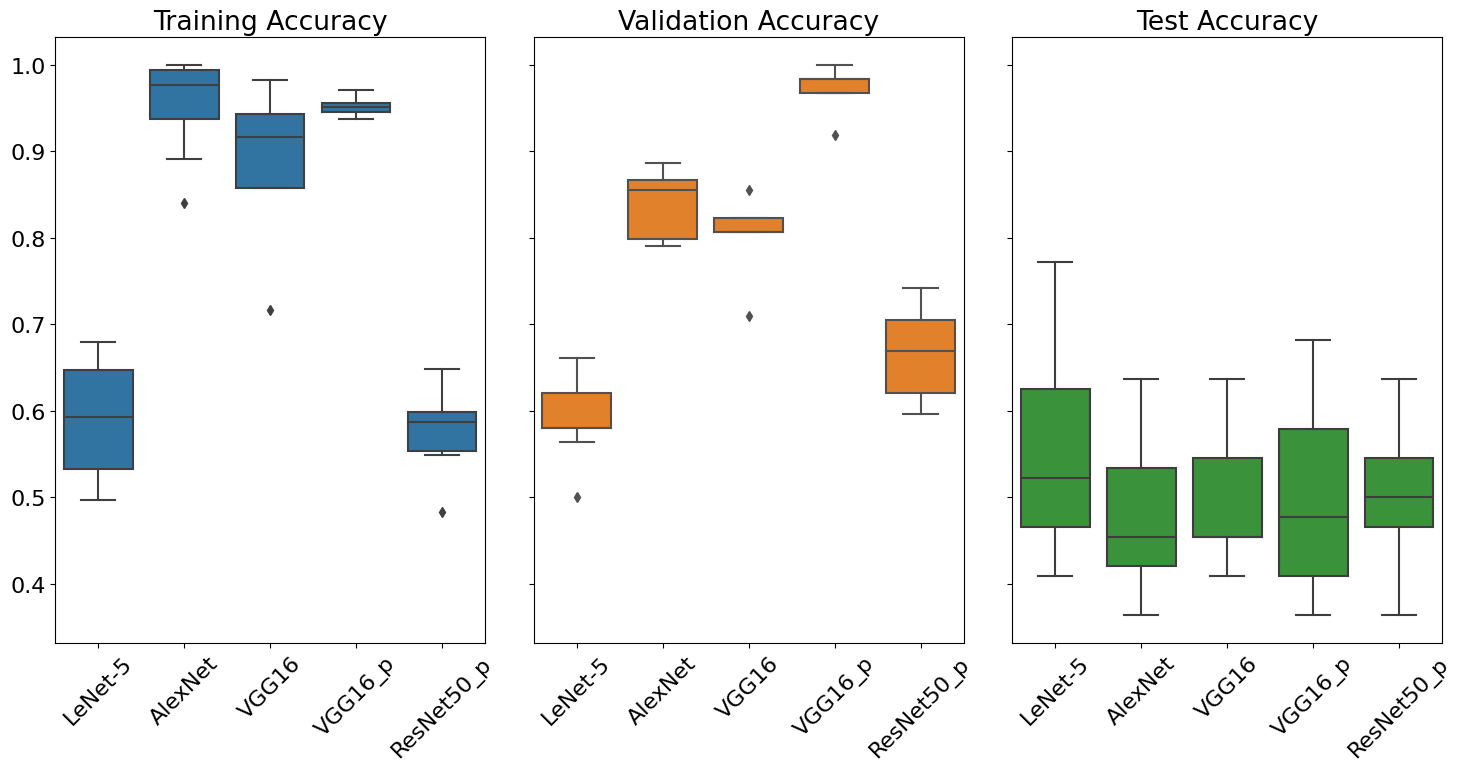
\includegraphics[width=\textwidth]{./tex_images/bootstrap_results.png}
    \caption{Results of first classification approach on the Kaggle dataset}
    \label{fig:Kaggle_results}
\end{figure}

Most of the models successfully learned the features of the training and validation datasets,
however on the test dataset all failed to classify the images in an acceptable level, mostly
achieving the level of a random classifier only.
This lead to the realization that the low number of images compared with the high variety of the track
failures will result in a situation where the model can easily learn the specifics of the training and
validation dataset preventing of any generalization to the test dataset.

As a followup a search for a more extended dataset and more refined models were started.
The company MÁV Central Rail And Track Inspection Ltd. (MÁV CRTI Ltd.) \cite{_mav_} was approached
as they are proficient in railway track inspection and have the equipment and data that could be used
for building such a model.

The expectation towards the dataset is to contain much more image than the set obtained from the
Kaggle webpage and the type of defect should be limited (for example only to surface defects).
The variance of the images should be narrowed down, for example the positioning, view angle or the
distance of the camera from the rails shall be restricted.

Due to the nature of the problem, any real life dataset is not expected to have any kind of annotation,
therefore the modeling approach needed to be change to unsupervised learning.
The problem statement refers to find certain defects of the rails, that is basically a result of a
deterioration process, which end up in a certain deviation from the normal condition.
This leads to the idea to apply anomaly detection models and try to identify the video frames
that contain such deviations.

\subsection{MÁV CRTI Ltd.}
The MÁV CRTI Ltd. was established in 1996 by MÁV Hungarian State Railways Co.
The scope of the company covers the fields of technical inspection and analysis related
railway tracks, rails and corresponding structures:
\begin{itemize}
    \item Geometric measurement of tracks and geometric condition survey
    \item Measurement, examination and qualification of railway rails
    \item Qualification of new and used superstructure materials
    \item Examination of bridges
    \item Examination of substructures
    \item Development related to rail measurement, examination and line maintenance
\end{itemize}

A comprehensive overview about the company, it's activities and history can be found at
\cite{_mav_} and in \cite{kfv_25years}.

The Rail Diagnostic Department carries out regular measurements on the railway tracks in order
to determine the overall condition of the rails and thus ensuring the safety of railway operation.
These inspections are carried out by special railway measurement equipment and inspection vehicles,
Starting from the simplest visual inspections carried out by the maintenance personnel up to
special ultrasonic examinations and rail profile measurements.
With such equipment rail surface and internal defects can be detected and detailed information about
the track profile can be obtained along hundreds of kilometers of railway tracks.

The Rail Diagnostic Department already has some experience with machine learning based rail
defect detection providing options for benchmarking the models created through this project.
It also reflects the importance of such approach, as today visual inspection demands heavy efforts
let that be the work done by the maintenance personnel (intrinsically walking along the tracks)
or the monitoring of the video footage taken during the inspection rides.

Currently, MÁV CRTI Ltd. operates two vehicles for rail inspection purposes, the SDS and FMK-008 shown on
Figure \ref{fig:vehicles}, both equipped with different measurement and inspection systems.
Fortunately both of them is equipped with video recording, however with different systems.
After a first view on the video files the system of the SDS vehicle is selected for a first modelling
approach.

\begin{figure}[!ht]
    \centering
    \begin{subfigure}{0.45\textwidth}
        \centering
        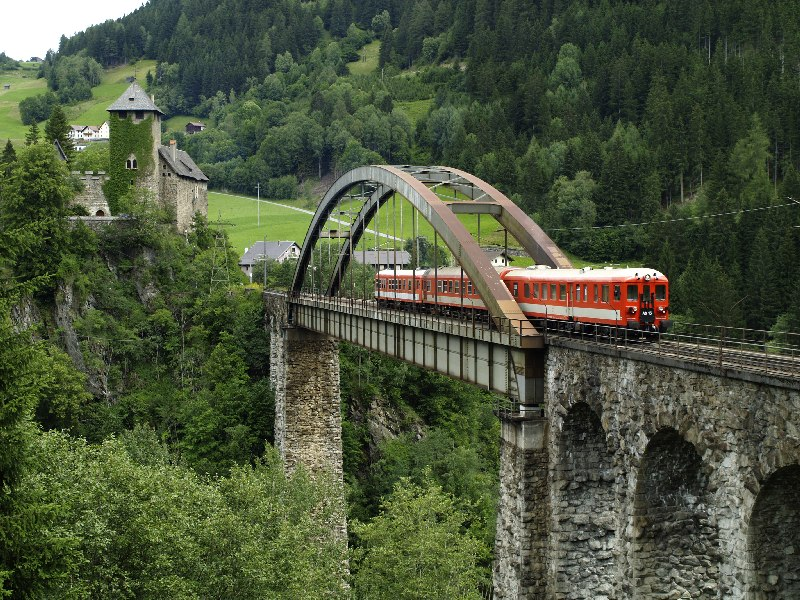
\includegraphics[height=3cm]{./tex_images/sds.jpg}
        \caption*{SDS}
    \end{subfigure}
    \begin{subfigure}{0.45\textwidth}
        \centering
        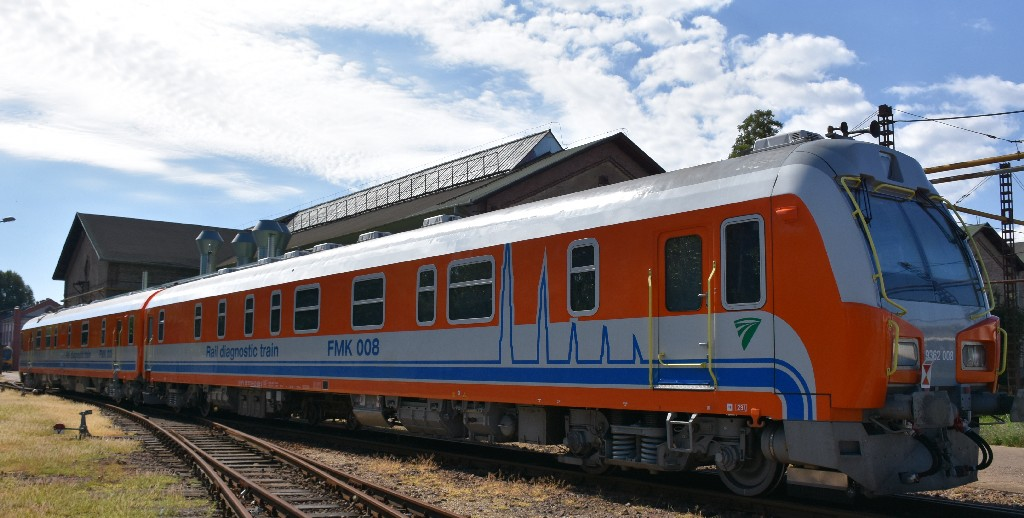
\includegraphics[height=3cm]{./tex_images/FMK008.jpg}
        \caption*{FMK-008}
    \end{subfigure}
    \caption{Railway inspection vehicles of MÁV CRTI Ltd.}
    \label{fig:vehicles}
\end{figure}

\subsection{Modelling approach and problem statement}
During the first part of the project convolutional neural networks with classification head were applied
on annotated dataset.
A step forward was taken by obtaining real world data, however this comes with the burden of
missing labeling.
Therefore, the modeling approach was also changed from supervised learning to unsupervised learning.

Autoencoders form a subgroup of algorithms of unsupervised learning.
The main target of such models is to reconstruct the original input on the output.
The basic idea behind an Autoencoder model is to generate feature vectors from the input
dataset (encode the dataset), this is the so-called Encoder part.
This set of feature vectors, called as latent space contains the representation of the dataset.
In the second part, the Decoder parts tries to recreate the input data based on the feature vector
generated by the Encoder.
In current use case this means that the single images of the rail is translated to feature vectors
and then the original image is recreated with some error using the Decoder.

The general structure of Autoencoders is shown in Figure \ref{fig:autoencoder}.

\begin{figure}[!ht]
    \centering
    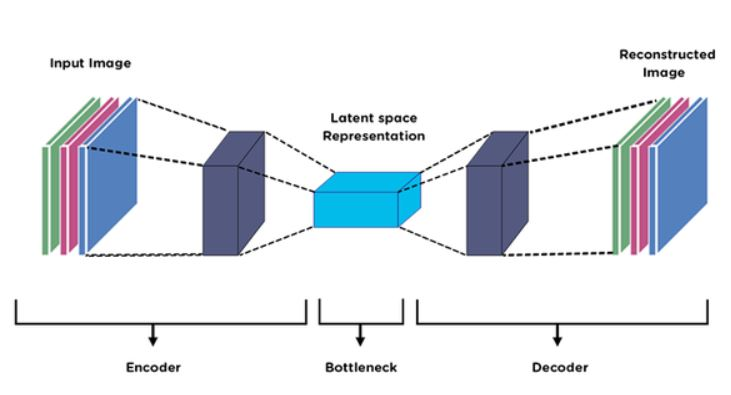
\includegraphics[width=0.6\textwidth,trim={0 0 0 1cm},clip]{./tex_images/autoencoder.jpeg}
    \caption{General structure of Autoencoders \cite{khosla_auto_2021}}
    \label{fig:autoencoder}
\end{figure}

A comprehensive overview about Deep Learning algorithms is given in \cite{Goodfellow-et-al-2016}.
Chapter 14 of this book explains the mathematical structure of Autoencoders.
Another introduction can be found at \cite{_autoencoder_2023}.

Autoencoders allow two basic type of anomaly detection methods.
First approach is to compare the input and output information, in general the autoencoder
can learn the features of the common images effectively, meaning that the decoded part will
be quite comparable with the input.
This means that the distance (or loss) defined between the input and output should be lower than
the case, when there is an outlier that contains features that are not seen by the model,
resulting in a not precise decomposition and decoding.

Secondly, the representation of the images stored in the latent space can be searched for outliers.
As rail defect happen very seldom, their feature vector should occur very rarely as well.
If the encoder is able to extract the differentiating features, then the outlier characteristics
can be preserved in the latent space.
Any general algorithm can be used to find these vectors, such as Isolation Forest, One-Class SVM or
Local Outlier Factor (please see \cite{_anomaly_2023} or \cite{sklearn_outlier_detection}
for additional examples).
Furthermore, the latent space can be clustered by any general clustering algorithm, for example:
DBSCAN, OPTICS, and so on, please refer to \cite{sklearn_clustering}.
These are also capable to identify outliers or clusters with limited number of elements.

In this way the problem was reformulated and traced back to anomaly detection, thus resulting in the
following key questions:

\begin{enumerate}[label=Q\arabic*]
    \item \label{itm:Q1} Can anomaly detection algorithms used to detect rail defects?
    \item \label{itm:Q2} What models could be applied on the given dataset?
    \item \label{itm:Q3} What accuracy rate can be achieved with the models?
\end{enumerate}

\subsection{Structure of the document}
The Section \ref{dataset} gives a deep view on the sample dataset.
The structure of the models introduced in Section \ref{model}.
The realization of the models, structure of the software code is explained in Section \ref{sw_code}.
The results are interpreted in Section \ref{results} and discussed in Section \ref{discussion}.
Further steps and possible improvement options covered with a summary of the results in
Section \ref{conclusion}.